%%%%%%%%%%%%%%%%%%%%%%%%%%%%%%%%%%%%%%%%%%%%%%%%%%%%%%%%%%%%%%%%%%%%
%% I, the copyright holder of this work, release this work into the
%% public domain. This applies worldwide. In some countries this may
%% not be legally possible; if so: I grant anyone the right to use
%% this work for any purpose, without any conditions, unless such
%% conditions are required by law.
%%%%%%%%%%%%%%%%%%%%%%%%%%%%%%%%%%%%%%%%%%%%%%%%%%%%%%%%%%%%%%%%%%%%

\documentclass{beamer}
\usetheme[university=bs,faculty=standard]{fibeamer}
\usepackage[utf8]{inputenc}
\usepackage[
  main=italian, %% By using `italian`as the main locale
                %% instead of `english`, you can typeset the
                %% presentation in Italian.
  english       %% The additional key allow foreign texts to be
]{babel}        %% typeset as follows:
%%
%%   \begin{otherlanguage}{italian}   ... \end{otherlanguage}
%%
%% These macros specify information about the presentation
\title{Implementazione in F\# di una procedura di refutazione per le logiche di G\"odel-Dummett} %% that will be typeset on the
%\subtitle{Presentation Subtitle} %% title page.
\author{Samuele Orfei}

%% These additional packages are used within the document:
\usepackage{ragged2e}  % `\justifying` text
\usepackage{booktabs}  % Tables
\usepackage{tabularx}
\usepackage{tikz}      % Diagrams
\usetikzlibrary{calc, shapes, backgrounds}
\usepackage{amsmath, amssymb}
\usepackage{url}       % `\url`s
\usepackage{listings}  % Code listings
\usepackage{graphicx}

\frenchspacing
\begin{document}
\frame[c]{\maketitle}

\begin{darkframes}

    \section{Presentazione}

    \subsection{Introduzione}
    \begin{frame}{Introduzione}

        \begin{block}{Le logiche $GD_k$ e $GD$}
            $GD_k$ è l'insieme di formule valide nei modelli lineari $K$, tali che $h(K) \leq k$, quindi $GD = \bigcap_{k \geq 0}GD_k$.

            $IPL \subset GD \subset \dots \subset GD_2 \subset GD_1 \subset GD_0 = CPL$, dove:
            \begin{itemize}
                \item $CPL$ è l'insieme delle formule valide nella logica classica
                \item $IPL$ è la logica intuizionista proposizionale
            \end{itemize}


        \end{block}

        Il punto di interesse principale del progetto sono le logiche di G\"odel-Dummett. \\
        Si tratta di una famiglia infinita di logiche dette \textit{intermedie}, caratterizzate da modelli lineari (di qualunque profondità). \\
        Per tali logiche sono noti vari calcoli e strategie di derivazione.

    \end{frame}

    \subsection{Obiettivo}
    \begin{frame}{Obiettivo}

        Si vuole definire un algoritmo, e la sua implementazione, che ha come obiettivo quello di definire un calcolo logico in grado di dimostrare la non-validità di una formula in ciascuna delle logiche di G\"odel-Dummett.\\

    \end{frame}

    \subsection{Teoria}

    \begin{frame}{Definizioni}
        \begin{block}{Calcolo di refutazione}
            Il calcolo $RGD_k(G)$ è un procedimento per inferire la non-provabilità di $G$ in $GD_k$, pensato per supportare una \textit{forward proof search}.
        \end{block}
        \begin{itemize}
            \item Data una logica $L$ ed una formula $A$, se si costruisce una derivazione di $A$ nel calcolo per $L$, allora la formula $A$ non è valida nella logica $L$.
            \item Dalla derivazione è possibile ottenere un \textit{contro-modello} per $A$, ossia un modello nella logica $L$ in cui $A$ è falsificata.
        \end{itemize}
    \end{frame}

    \begin{frame}{Definizioni}
        \begin{block}{Regole del calcolo}
            \begin{itemize}
                \item Regola sinistra: $\Gamma \not\Rightarrow_k \Lambda; \Delta \rightarrow A \supset B, \Gamma \not\Rightarrow_k \Lambda; \Delta$
                \item Regola destra: $\Gamma \not\Rightarrow_k \Lambda; \Delta \rightarrow \Gamma \not\Rightarrow_k \Lambda; \Delta, A \supset B$
                \item Regola successore: $\Gamma \not\Rightarrow_k \Lambda; \Delta \rightarrow \Gamma \setminus \Lambda^{'} \not\Rightarrow_{k+1} \Lambda^{'}; \Delta, \Lambda$
                \item Condizioni di termininazione: generazione di $\Gamma \not\Rightarrow_k \Lambda; \Delta$ con $G \in Cl^-(\Delta \cup \Lambda)$
            \end{itemize}
        \end{block}
    \end{frame}

    \subsection{Requisiti}
    \begin{frame}{Requisiti}

        \textbf{Requisiti di base}
        \begin{itemize}
            \item Lettura della formula sotto forma di stringa.
            \item Costruzione dell'albero di sintassi (rappresentazione interna).
            \item Applicazione del calcolo di refutazione e costruzione della derivazione, se possibile.
            \item Stampa a video dei passaggi fondamentali della derivazione.
        \end{itemize}

        \textbf{Requisiti sui tipi}
        \begin{itemize}
            \item Supporto degli operatori logici $\land$, $\lor$, $\supset$, $\neg$.
            \item Supporto di proposizioni atomiche e di costanti come $\bot$.
            \item Supporto di formule innestate.
        \end{itemize}

    \end{frame}

    \subsection{Requisiti}
    \begin{frame}{Requisiti}
        Le caratteristiche dei moduli e dell'algoritmo:
        \begin{itemize}
            \item Implementato in F\# compatibile con .NET 7.0.
            \item Modularità: possibilità di riutilizzare il codice.
            \item Tracciamento: in caso di errore, restituizione di errore con informazioni di traccia.
        \end{itemize}
    \end{frame}

    \subsection{Struttura del progetto}
    \begin{frame}{Struttura del progetto}
        \begin{itemize}
            \item Modulo \textit{Lexer} che mediante una grammatica restituisce una lista di \textit{Token} partendo dalla formula.
            \item Modulo \textit{Parser} che genera l'albero di sintassi della rappresentazione interna.
            \item Modulo \textit{Expression} per manipolare, trasformare o estrarre dati da una data formula.
            \item Modulo \textit{Calculus} che racchiude le funzioni che rappresentano il calcolo di refutazione.
        \end{itemize}
    \end{frame}

    \begin{frame}{Struttura del progetto}
        \begin{figure}[h]
            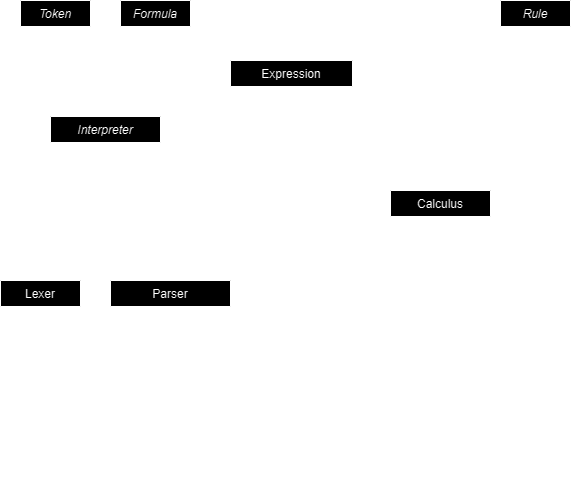
\includegraphics[scale=0.4]{../images/composizione.drawio.png}
        \end{figure}
    \end{frame}

    \subsection{Strumenti}
    \begin{frame}{Strumenti}
        \framesubtitle{Strumenti essenziali}
        \begin{itemize}
            \item F\#
            \item .NET Framework
        \end{itemize}
    \end{frame}

    \begin{frame}{Strumenti}
        \framesubtitle{Altri strumenti importanti}
        \begin{itemize}
            \item Librerie utilizzate durante lo sviluppo (List, Set, Map)
            \item IDE e/o editor di testo (Visual Studio Code)
            \item Versionamento (Github)
        \end{itemize}
    \end{frame}

    \begin{frame}{Strumenti}
        \begin{figure}[h]
            \caption{Funzionamento del .NET runtime, dal web.}
            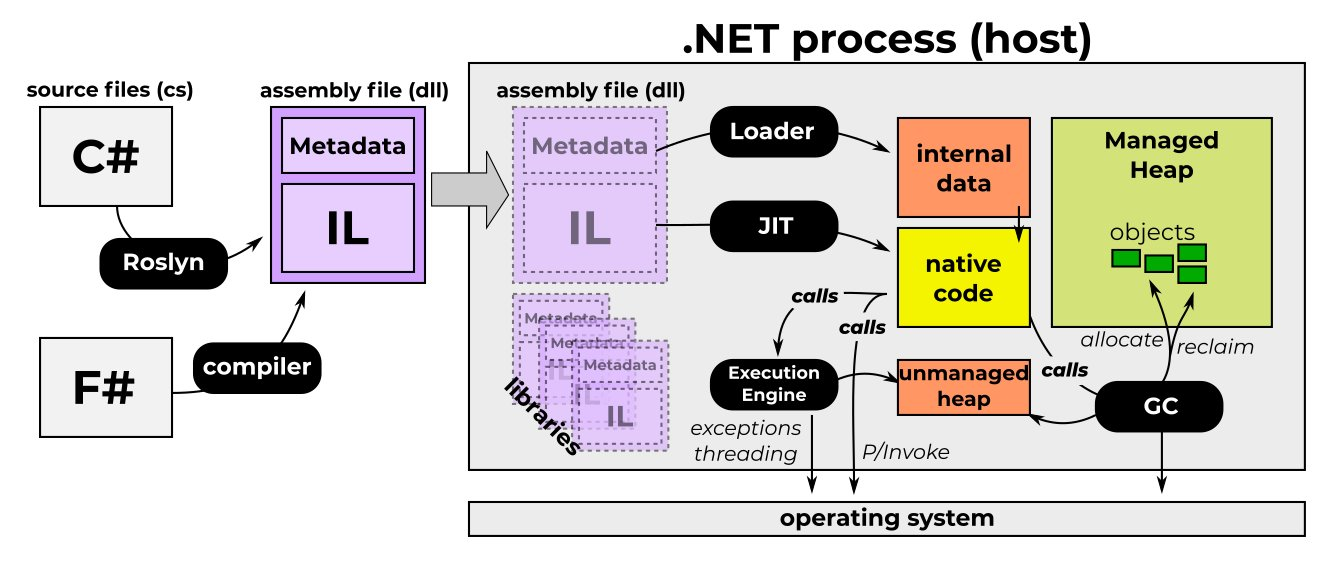
\includegraphics[width=\textwidth]{../images/dotnet.png}
        \end{figure}
    \end{frame}

    \subsection{Conclusioni}
    \begin{frame}{Conclusioni}
        \textbf{Stato del progetto}
        \begin{itemize}
            \item Algoritmo completato
        \end{itemize}
        \textbf{Prospettive future}
        \begin{itemize}
            \item Miglioramento dell'interprete ed espansione della grammatica supportata
            \item Ottimizzazione del calcolo stesso
        \end{itemize}
    \end{frame}

    \begin{frame}{Conclusioni}
        \textbf{Grazie per l'attenzione.}
    \end{frame}

\end{darkframes}

\end{document}